\documentclass[12pt]{jarticle}
\usepackage{TUSIReport}
\usepackage{otf}
\usepackage[dvipdfmx]{graphicx}
\usepackage[dvipdfmx]{color}
\usepackage{amsmath}
\usepackage{amssymb}
\usepackage{color}
\usepackage{hhline}
\usepackage{fancybox,ascmac}
\usepackage{multirow}
\usepackage{url}
\usepackage{bm}
\usepackage{listings,jlisting}
\lstdefinestyle{log}{
    frame={tblr},
    basicstyle={\footnotesize},
    tabsize={4},
}
\lstdefinestyle{lstR}{
    language={R},
    backgroundcolor={\color[gray]{.85}},
    basicstyle={\small},
    identifierstyle={\small},
    commentstyle={\small\ttfamily \color[rgb]{0,0.5,0}},
    keywordstyle={\small\bfseries \color[rgb]{1,0,0}},
    ndkeywordstyle={\small},
    stringstyle={\small\ttfamily \color[rgb]{0,0,1}},
    frame={tb},
    breaklines=true,
    columns=[l]{fullflexible},
    numbers=left,
    xrightmargin=0zw,
    xleftmargin=3zw,
    numberstyle={\scriptsize},
    stepnumber=1,
    numbersep=1zw,
    morecomment=[l]{//}
}
\begin{document}
%%%%%%%%%%%%%%%%%%%%%%%%%%%%%%%%%%%%%%%%%%%%%%%%%%%%%%%%%%%%%%
% 表紙を出力する場合は,\提出者と\共同実験者をいれる
% \提出者{科目名}{課題名}{提出年}{提出月}{提出日}{学籍番号}{氏名}
% \共同実験者{一人目}{二人目}{..}{..}{..}{..}{..}{八人目}
%%%%%%%%%%%%%%%%%%%%%%%%%%%%%%%%%%%%%%%%%%%%%%%%%%%%%%%%%%%%%%
\提出者{情報工学実験2}{実験テーマ4 統計的推測と単回帰分析}{2020}{9}{28}{4619055}{辰川力駆}
\共同実験者{}{}{}{}{}{}{}{}

%%%%%%%%%%%%%%%%%%%%%%%%%%%%%%%%%%%%%%%%%%%%%%%%%%%%%%%%%%%%%%
% 表紙を出力しない場合は,以下の「\表紙出力」をコメントアウトする
%%%%%%%%%%%%%%%%%%%%%%%%%%%%%%%%%%%%%%%%%%%%%%%%%%%%%%%%%%%%%%
\表紙出力

%%%%%%%%%%%%%%%%%%%%%%%%%%%%%%%%%%%%%%%%%%%%%%%%%%%%%%%%%%%%%%
% 以下はレポート本体である.別途 TeXファイルを作成し \input 使っても良い
%%%%%%%%%%%%%%%%%%%%%%%%%%%%%%%%%%%%%%%%%%%%%%%%%%%%%%%%%%%%%%

\section{はじめに}
本実験では、単回帰分析の考え方と手順を理解することを目標とする。

\section{目的}
\begin{itemize}
    \item [1.]単回帰分析の考え方と手順

          単回帰分析の目的、考え方、手順を理解する
    \item [2.]単回帰分析における行列表現

          単回帰分析における行列表現(線形回帰モデル、正規方程式、最小二乗推定量など)
          を理解する
    \item [3.]実際のデータ解析

          実際のデータに回帰分析を適用することで、解析法を実践的に利用・応用できるようにする
\end{itemize}

\section{実験方法}
\subsection{実験1 単回帰分析の考え方と手順}
6つの市町村の人口と行政職員数の仮想データを表1に示す。
また、各市町村の人口を$x_i$,職員数を$y_i(i=1,...,n(=6))$と表記する。

\begin{table}[htb]
    \begin{center}
        \caption{市町村の人口と行政職員数}
        \begin{tabular}{|c|c|c|} \hline
            市町村 & 人口$x$(千人) & 職員数$y$(人) \\ \hline
            A      & 1             & 10            \\
            B      & 2             & 20            \\
            C      & 3             & 20            \\
            D      & 3             & 40            \\
            E      & 5             & 40            \\
            F      & 1             & 5             \\ \hline
            合計   & 15            & 135           \\\hline
        \end{tabular}
    \end{center}
\end{table}

\begin{itemize}
    \item [1.]次の統計量を計算する。
          \begin{eqnarray}
              \sum_{i=1}^{n} x_i, \sum_{i=1}^{n} y_i, \sum_{i=1}^{n} {x_i}^2, \sum_{i=1}^{n} {y_i}^2, \sum_{i=1}^{n} x_iy_i \nonumber
          \end{eqnarray}
    \item [2.]次式が整理することを証明する。
          \begin{eqnarray}
              \sum_{i=1}^{n} (x_i-\bar{x})^2&=&\sum_{i=1}^{n} {x_i}^2-n\bar{x}^2 \\
              \sum_{i=1}^{n} (y_i-\bar{y})^2&=&\sum_{i=1}^{n} {y_i}^2-n\bar{y}^2 \\
              \sum_{i=1}^{n} (x_i-\bar{x})(y_i-\bar{y})&=&\sum_{i=1}^{n} {x_iy_i}-n\bar{xy}
          \end{eqnarray}
    \item [3.]人口$x$と職員数$y$の基本統計量(データ数、平均、標準偏差、最小値、最大値)を計算する。
          \begin{eqnarray}
              人口xの平均&=&\bar{x}=\frac{\sum_{i=1}^{n} x_i}{n} \nonumber\\
              人口xの標準偏差&=&\sqrt{\frac{\sum_{i=1}^{n} (x_i-\bar{x})^2}{n-1}}=\sqrt{\frac{\sum_{i=1}^{n} {x_i}^2-n\bar{x}^2}{n-1}} \nonumber\\
              職員数yの平均&=&\bar{y}=\frac{\sum_{i=1}^{n} y_i}{n} \nonumber\\
              職員数yの標準偏差&=&\sqrt{\frac{\sum_{i=1}^{n} (y_i-\bar{y})^2}{n-1}}=\sqrt{\frac{\sum_{i=1}^{n} {y_i}^2-n\bar{y}^2}{n-1}} \nonumber
          \end{eqnarray}
    \item [4.]人口$x$と職員数$y$のPearsonの積率相関係数$r$を計算する。
          \begin{eqnarray}
              r=\frac{\sum_{i=1}^{n} (x_i-\bar{x})(y_i-\bar{y})}{\sqrt{\sum_{i=1}^{n} (x_i-\bar{x})^2} \sqrt{\sum_{i=1}^{n} (y_i-\bar{y})^2}}=\frac{\sum_{i=1}^{n} {x_iy_i}-n\bar{xy}}{\sqrt{\sum_{i=1}^{n} (x_i-\bar{x})^2} \sqrt{\sum_{i=1}^{n} (y_i-\bar{y})^2}}
          \end{eqnarray}
    \item [5.]人口$x$を横軸,職員数$y$を縦軸にした散布図を作成して、両者の関係を調べる。
    \item [6.]単回帰モデル$y_i=\beta_0+\beta_1 x_i + \varepsilon_i(i=1,...,n)$をあてはめる。
          $\beta_0$と$\beta_1$の推定量を$\hat{\beta_0}$と$\hat{\beta_1}$とすると、
          目的変数(応答変数)である職員数の予測値は$\hat{y_i}=\hat{\beta_0}+\hat{\beta_1}x_i$で
          与えられる。
          次式の残差平方和$S_e$を$\hat{\beta_0}$と$\hat{\beta_1}$でそれぞれ偏微分する。
          \begin{eqnarray}
              S_e=\sum_{i=1}^{n} (y_i-\hat{y_i})^2 = \sum_{i=1}^{n} (y_i-(\hat{\beta_0}+\hat{\beta_1}x_i))^2
          \end{eqnarray}
    \item [7.]正規方程式を作成する。
    \item [8.]正規方程式を解き、$\beta_0$と$\beta_1$の最小二乗推定量を数式で表現する。
    \item [9.]最小二乗推定量$\hat{\beta_0}$,$\hat{\beta_1}$の値を求める。
    \item [10.]得られた回帰直線($\hat{y_i}=\hat{\beta_0}+\hat{\beta_1}x_i$)を
          手順5で作成した散布図に図示して、結果を考察する。
    \item [11.]データ分析[回帰分析]を用いて、これまでに得られた結果と同様の結果が得られることを確認する。
\end{itemize}

\clearpage

\subsection{実験2 単回帰分析における行列表現}
データ数を$n$とする。
目的変数ベクトル$\bm Y$と説明変数を含む定数行列$\bm X$を次式で定義する。
\[
    \bm Y = \left(
    \begin{array}{c}
            y_1    \\
            y_2    \\
            \vdots \\
            y_n
        \end{array}
    \right)
\]
\[
    \bm X = \left(
    \begin{array}{cc}
            1      & x_1    \\
            1      & x_2    \\
            \vdots & \vdots \\
            1      & x_n
        \end{array}
    \right)
\]
このとき、実験1の単回帰モデルは
\begin{eqnarray}
    \bm y=\bm X \bm \beta+ \bm \varepsilon \nonumber
\end{eqnarray}
で与えられる。ここで$\bm \beta$は母回帰係数,$ \bm \varepsilon$は誤差ベクトルであり、
次式で定義される。

\[
    \bm \beta = \left(
    \begin{array}{c}
            \beta_0 \\
            \beta_1
        \end{array}
    \right)
\]
\[
    \bm \varepsilon = \left(
    \begin{array}{c}
            \varepsilon_0 \\
            \varepsilon_1 \\
            \vdots        \\
            \varepsilon_n
        \end{array}
    \right)
\]
$\bm \beta$の推定量を$\hat{\bm \beta}=(\hat{\beta_0},\hat{\beta_1})^T$とする。
\begin{enumerate}
    \item 残差平方和$S_e$を行列で表現する。
    \item 残差平方和$S_e$を$\hat{\bm \beta}$で微分し、正規方程式を導く。
    \item 正規方程式から最小二乗推定量が
          \begin{eqnarray}
              \hat{\bm \beta}=(\bm X^T \bm X)^{-1} \bm X^T \bm y
          \end{eqnarray}
          で得られることを確認する。
    \item ベクトル$\bm Y$と行列$\bm X$を定義する。
          \clearpage
    \item 次の値を計算する。
          \begin{itemize}
              \item [(a)]$x$の平均$\bar{x}$
              \item [(b)]$y$の平均$\bar{y}$
              \item [(c)]$x$の偏差平方和$\bar{x}=\sum_{i=1}^{n} (x_i-\bar{x})^2$
              \item [(d)]$y$の偏差平方和$\bar{y}=\sum_{i=1}^{n} (y_i-\bar{y})^2$
          \end{itemize}
    \item 次の値を計算する。
          \begin{itemize}
              \item [(a)]最小二乗推定量 $\hat{\bm \beta}=(\bm X^T \bm X)^{-1} \bm X^T \bm Y$
              \item [(b)]予測値$\hat{\bm Y}=\bm X \hat{\bm \beta}$
              \item [(c)]残差$\bm Y-\hat{\bm Y}$
          \end{itemize}
    \item 射影行列$\bm H = \bm X (\bm X^T \bm X)^{-1}\bm X^T$を計算し、次式が成り立つことを確認する。
          \begin{itemize}
              \item [(a)]対称性$\bm H^T=\bm H$
              \item [(b)]べき等性$\bm H \bm H = \bm H$
              \item [(c)]$trace(\bm H)= 2$(パラメータ数)
          \end{itemize}
    \item 得られた最小二乗推定量のもとで、総平方和、モデル平方和、残差平方和を計算し
          \begin{eqnarray}
              総平方和=モデル平方和+残差平方和
          \end{eqnarray}
          が成り立つことを確認する。
    \item 寄与率(決定係数)= モデル平方和/総平方和を計算し、モデルの当てはまりを評価する。
\end{enumerate}

\clearpage

\section{結果・考察・課題}
\subsection{実験1 単回帰分析の考え方と手順}
\begin{shadebox}
    \fbox{課題1}実験1の結果をまとめる。
\end{shadebox}
\begin{itemize}
    \item [1.]計算すると次のようになった。
          \begin{eqnarray}
              \sum_{i=1}^{n} x_i&=&15 \nonumber\\
              \sum_{i=1}^{n} y_i&=&135 \nonumber\\
              \sum_{i=1}^{n} {x_i}^2&=&49 \nonumber\\
              \sum_{i=1}^{n} {y_i}^2&=&4125 \nonumber\\
              \sum_{i=1}^{n} x_iy_i&=&435 \nonumber
          \end{eqnarray}
    \item [2.]式(1),(2),(3)が成り立つことを示す。式(1)の左辺を変形すると、
          \begin{eqnarray}
              \sum_{i=1}^{n} (x_i-\bar{x})^2&=&\sum_{i=1}^{n} (x_i^2-2x_i\bar{x}+\bar{x}^2) \nonumber\\
              &=&\sum_{i=1}^{n} x_i^2-\sum_{i=1}^{n} 2x_i\bar{x}+n\bar{x}^2 \nonumber\\
              &=&\sum_{i=1}^{n} x_i^2-\sum_{i=1}^{n} 2\bar{x}^2+n\bar{x}^2 \nonumber \\
              &=&\sum_{i=1}^{n} x_i^2-2n\bar{x}^2+n\bar{x}^2 \nonumber \\
              &=&\sum_{i=1}^{n} x_i^2-n\bar{x}^2 \nonumber
          \end{eqnarray}
          となり、右辺と一致する。
          同様にして、式(2)の左辺を変形すると、下記のようになり右辺と一致する。
          \begin{eqnarray}
              \sum_{i=1}^{n} (y_i-\bar{y})^2&=&\sum_{i=1}^{n} (y_i^2-2y_i\bar{y}+\bar{y}^2) \nonumber\\
              &=&\sum_{i=1}^{n} y_i^2-2n\bar{y}^2+n\bar{y}^2 \nonumber \\
              &=&\sum_{i=1}^{n} y_i^2-n\bar{y}^2 \nonumber
          \end{eqnarray}
          式(3)も同様の考え方より、
          \begin{eqnarray}
              \sum_{i=1}^{n} (x_i-\bar{x})(y_i-\bar{y})&=& \sum_{i=1}^{n} (x_iy_i-x_i\bar{y}-y_i\bar{x}+\bar{x}\bar{y}) \nonumber \\
              &=& \sum_{i=1}^{n} x_iy_i-n\bar{x}\bar{y}-n\bar{x}\bar{y}+n\bar{x}\bar{y} \nonumber \\
              &=&   \sum_{i=1}^{n} {x_iy_i}-n\bar{xy} \nonumber
          \end{eqnarray}
          となり、証明できた。

    \item [3.]データの数は$x$,$y$どちらも、6つである。残りの基本統計量(平均、標準偏差、最小値、最大値)は以下のようになった。
          \begin{table}[htb]
              \begin{center}
                  \caption{人口と行政職員数の基本統計量}
                  \begin{tabular}{|c|c|c|} \hline
                      基本統計量 & 人口$x$(千人) & 職員数$y$(人) \\ \hline
                      平均       & 2.5           & 22.5          \\
                      標準偏差   & 1.52          & 14.75         \\
                      最小値     & 1             & 5             \\
                      最大値     & 5             & 40            \\ \hline
                  \end{tabular}
              \end{center}
          \end{table}


    \item [4.]Pearsonの積率相関係数$r$は式(4)より、次のようになった。
          \begin{eqnarray}
              r&=&\frac{\sum_{i=1}^{n} (x_i-\bar{x})(y_i-\bar{y})}{\sqrt{\sum_{i=1}^{n} (x_i-\bar{x})^2} \sqrt{\sum_{i=1}^{n} (y_i-\bar{y})^2}} \nonumber\\
              &\fallingdotseq &0.87 \nonumber
          \end{eqnarray}

    \item [5.]散布図を作成すると、次のようになった(後述の手順10の直線を含む)。
          \begin{figure}[h]
              \begin{center}
                  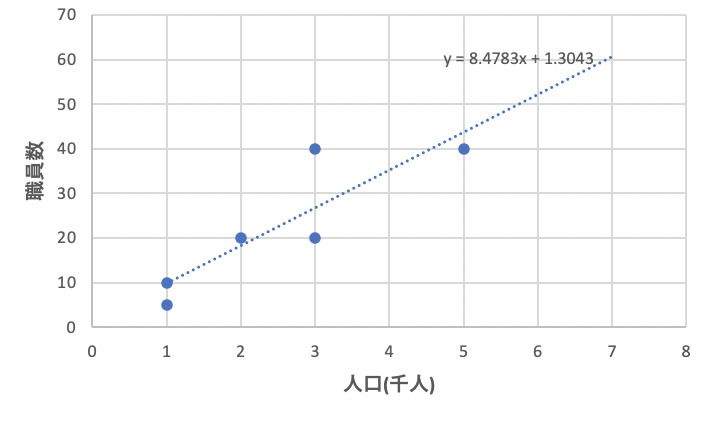
\includegraphics[scale=0.7]{kadai4_2_fig1.png}
              \end{center}
              \caption{人口と行政職員数の散布図}
          \end{figure}
          \clearpage

    \item [6.]式(5)の残差平方和$S_e$を$\hat{\beta_0}$と$\hat{\beta_1}$でそれぞれ偏微分すると、
          \begin{eqnarray}
              \frac{\partial S_e}{\partial \hat{\beta_0}}&=& \frac{\partial}{\partial \hat{\beta_0}}\sum_{i=1}^{n} (y_i-(\hat{\beta_0}+\hat{\beta_1}x_i))^2 \nonumber \\
              &=& \frac{\partial}{\partial \hat{\beta_0}}\sum_{i=1}^{n} (-\hat{\beta_0}+(y_i-\hat{\beta_1}x_i))^2 \nonumber \\
              &=& -2\sum_{i=1}^{n} (-\hat{\beta_0}+(y_i-\hat{\beta_1}x_i)) \nonumber \\
              &=& 2\sum_{i=1}^{n} (\hat{\beta_0}-y_i+\hat{\beta_1}x_i) \nonumber \\
              &=& 2(n\hat{\beta_0}-\sum_{i=1}^{n}y_i+\hat{\beta_1}\sum_{i=1}^{n}x_i)
          \end{eqnarray}
          \begin{eqnarray}
              \frac{\partial S_e}{\partial \hat{\beta_1}}&=& \frac{\partial}{\partial \hat{\beta_1}}\sum_{i=1}^{n} (y_i-(\hat{\beta_0}+\hat{\beta_1}x_i))^2 \nonumber \\
              &=& \frac{\partial}{\partial \hat{\beta_1}}\sum_{i=1}^{n} (-\hat{\beta_1}x_i+(y_i-\hat{\beta_0}))^2 \nonumber \\
              &=& -2\sum_{i=1}^{n} (-\hat{\beta_1}x_i^2+(y_i-\hat{\beta_0})x_i) \nonumber \\
              &=& 2\sum_{i=1}^{n} (\hat{\beta_1}x_i^2-x_iy_i+\hat{\beta_0}x_i) \nonumber \\
              &=& 2(\hat{\beta_1}\sum_{i=1}^{n}x_i^2-\sum_{i=1}^{n} x_iy_i+\hat{\beta_0}\sum_{i=1}^{n} x_i)
          \end{eqnarray}
    \item [7.]式(8),(9)において、
          \begin{eqnarray}
              \frac{\partial S_e}{\partial \hat{\beta_0}} &=&0 \nonumber \\
              \frac{\partial S_e}{\partial \hat{\beta_1}}&=&0 \nonumber
          \end{eqnarray}
          とするのでそれぞれ整理すると、
          \begin{eqnarray}
              \frac{\partial S_e}{\partial \hat{\beta_0}} &=&0 \nonumber \\
              2(n\hat{\beta_0}-\sum_{i=1}^{n}y_i+\hat{\beta_1}\sum_{i=1}^{n}x_i)&=&0 \nonumber \\
              n\hat{\beta_0}-\sum_{i=1}^{n}y_i+\hat{\beta_1}\sum_{i=1}^{n}x_i &=&0 \nonumber \\
              \sum_{i=1}^{n}y_i&=&n\hat{\beta_0}+\hat{\beta_1}\sum_{i=1}^{n}x_i
          \end{eqnarray}
          \begin{eqnarray}
              \frac{\partial S_e}{\partial \hat{\beta_1}}&=&0 \nonumber \\
              2(\hat{\beta_1}\sum_{i=1}^{n}x_i^2-\sum_{i=1}^{n} x_iy_i+\hat{\beta_0}\sum_{i=1}^{n} x_i) &=&0 \nonumber \\
              \hat{\beta_1}\sum_{i=1}^{n}x_i^2-\sum_{i=1}^{n} x_iy_i+\hat{\beta_0}\sum_{i=1}^{n} x_i &=&0 \nonumber \\
              \sum_{i=1}^{n} x_iy_i &=&\hat{\beta_1}\sum_{i=1}^{n}x_i^2+\hat{\beta_0}\sum_{i=1}^{n} x_i
          \end{eqnarray}
          よって正規方程式ができた。
    \item [8.]式(10),(11)の連立方程式を解く。式(10)を変形すると、
          \begin{eqnarray}
              \sum_{i=1}^{n}y_i&=&n\hat{\beta_0}+\hat{\beta_1}\sum_{i=1}^{n}x_i \nonumber \\
              n\hat{\beta_0}&=& \sum_{i=1}^{n}y_i-\hat{\beta_1}\sum_{i=1}^{n}x_i \nonumber \\
              \hat{\beta_0}&=& \frac{\sum_{i=1}^{n}y_i-\hat{\beta_1}\sum_{i=1}^{n}x_i}{n}
          \end{eqnarray}
          となるので、式(12)を式(11)に代入すると、
          \begin{eqnarray}
              \sum_{i=1}^{n} x_iy_i &=&\hat{\beta_1}\sum_{i=1}^{n}x_i^2+\hat{\beta_0}\sum_{i=1}^{n} x_i \nonumber \\
              \sum_{i=1}^{n} x_iy_i &=&\hat{\beta_1}\sum_{i=1}^{n}x_i^2+ (\frac{\sum_{i=1}^{n}y_i-\hat{\beta_1}\sum_{i=1}^{n}x_i}{n})\sum_{i=1}^{n} x_i \nonumber \\
              n\sum_{i=1}^{n} x_iy_i &=&n\hat{\beta_1}\sum_{i=1}^{n}x_i^2+ (\sum_{i=1}^{n}y_i-\hat{\beta_1}\sum_{i=1}^{n}x_i)\sum_{i=1}^{n} x_i \nonumber \\
              n\sum_{i=1}^{n} x_iy_i &=&n\hat{\beta_1}\sum_{i=1}^{n}x_i^2+ \sum_{i=1}^{n} x_i\sum_{i=1}^{n}y_i-\hat{\beta_1}(\sum_{i=1}^{n}x_i)^2 \nonumber \\
              n\hat{\beta_1}\sum_{i=1}^{n}x_i^2-\hat{\beta_1}(\sum_{i=1}^{n}x_i)^2   &=&  n\sum_{i=1}^{n} x_iy_i-\sum_{i=1}^{n} x_i\sum_{i=1}^{n}y_i \nonumber \\
              \hat{\beta_1}\sum_{i=1}^{n}x_i^2-\hat{\beta_1}(\sum_{i=1}^{n}x_i)^2/n   &=&  \sum_{i=1}^{n} x_iy_i-\sum_{i=1}^{n} x_i\sum_{i=1}^{n}y_i/n \nonumber \\
              \hat{\beta_1}(\sum_{i=1}^{n}x_i^2-(\sum_{i=1}^{n}x_i)^2/n)   &=&  \sum_{i=1}^{n} x_iy_i-\sum_{i=1}^{n} x_i\sum_{i=1}^{n}y_i/n \nonumber \\
              \hat{\beta_1} &=&  \frac{\sum_{i=1}^{n} x_iy_i-\sum_{i=1}^{n} x_i\sum_{i=1}^{n}y_i/n}{\sum_{i=1}^{n}x_i^2-(\sum_{i=1}^{n}x_i)^2/n}
          \end{eqnarray}

          \clearpage
          また、$\hat{y_i}=\hat{\beta_0}+\hat{\beta_1}x_i$を用いて、
          \begin{eqnarray}
              \sum_{i=1}^{n}\hat{y_i}&=&\sum_{i=1}^{n}\hat{\beta_0}+\sum_{i=1}^{n}\hat{\beta_1}x_i \nonumber \\
              n\bar{y}&=&n\hat{\beta_0}+n\hat{\beta_1}\bar{x} \nonumber \\
              \bar{y}&=&\hat{\beta_0}+\hat{\beta_1}\bar{x} \nonumber \\
              \hat{\beta_0}&=& \bar{y}-\hat{\beta_1}\bar{x}
          \end{eqnarray}
          となり、最小二乗推定量$\hat{\beta_0}$,$\hat{\beta_1}$を数式で表現することができた。
    \item [9.]式(13),(14)に求めた統計量を代入すると
          \begin{eqnarray}
              \hat{\beta_0}&=& 1.3043 \nonumber \\
              \hat{\beta_1}&=& 8.4783 \nonumber
          \end{eqnarray}
          となり、最小二乗推定量$\hat{\beta_0}$,$\hat{\beta_1}$の値を求めることができた。
    \item [10.]図1の散布図に直線を図示した。データ数は少ないが、直線の傾きより、人口と行政職員数で正の相関があると言える。
    \item [11.]データ分析[回帰分析]を用いると、下記のようになり、同様の結果を得ることができた。
          \begin{table}[htb]
              \begin{center}
                  \caption{人口と行政職員数の回帰分析}
                  \begin{tabular}{|c|c|c|} \hline
                      回帰統計 & 数値   \\ \hline
                      重相関 R & 0.87   \\
                      \hline  \hline
                               & 係数   \\\hline
                      切片     & 1.3043 \\ \hline
                      X 値 1   & 8.4783 \\ \hline
                  \end{tabular}
              \end{center}
          \end{table}
\end{itemize}

\begin{shadebox}
    \fbox{課題2}公表されてるデータ(標本数が50以上)を集めて、回帰分析を適用し、結果を考察する。
\end{shadebox}

\clearpage
\begin{table}[htb]
    \begin{center}
        \caption{労働力人口のデータ}
        \begin{tabular}{|c|c|c||c|c|c|} \hline
            年月         & 男(万人) & 女(万人) & 年月         & 男(万人) & 女(万人) \\\hline
            平成28年1月  & 3784     & 2896     & 平成30年5月  & 3816     & 3008     \\
            平成28年2月  & 3774     & 2874     & 平成30年6月  & 3816     & 2997     \\
            平成28年3月  & 3758     & 2871     & 平成30年7月  & 3809     & 3010     \\
            平成28年4月  & 3774     & 2869     & 平成30年8月  & 3811     & 3023     \\
            平成28年5月  & 3780     & 2871     & 平成30年9月  & 3815     & 3021     \\
            平成28年6月  & 3784     & 2900     & 平成30年10月 & 3822     & 3034     \\
            平成28年7月  & 3783     & 2910     & 平成30年11月 & 3843     & 3039     \\
            平成28年8月  & 3782     & 2905     & 平成30年12月 & 3830     & 3022     \\
            平成28年9月  & 3781     & 2900     & 平成31年1月  & 3810     & 3033     \\
            平成28年10月 & 3788     & 2897     & 平成31年2月  & 3829     & 3044     \\
            平成28年11月 & 3784     & 2899     & 平成31年3月  & 3836     & 3057     \\
            平成28年12月 & 3799     & 2915     & 平成31年4月  & 3822     & 3050     \\
            平成29年1月  & 3795     & 2916     & 令和元年5月  & 3820     & 3046     \\
            平成29年2月  & 3772     & 2901     & 令和元年6月  & 3824     & 3046     \\
            平成29年3月  & 3769     & 2898     & 令和元年7月  & 3829     & 3050     \\
            平成29年4月  & 3777     & 2918     & 令和元年8月  & 3834     & 3056     \\
            平成29年5月  & 3786     & 2938     & 令和元年9月  & 3827     & 3069     \\
            平成29年6月  & 3782     & 2947     & 令和元年10月 & 3834     & 3082     \\
            平成29年7月  & 3792     & 2947     & 令和元年11月 & 3839     & 3075     \\
            平成29年8月  & 3793     & 2953     & 令和元年12月 & 3836     & 3085     \\
            平成29年9月  & 3793     & 2951     & 令和2年1月   & 3835     & 3067     \\
            平成29年10月 & 3786     & 2946     & 令和2年2月   & 3839     & 3072     \\
            平成29年11月 & 3775     & 2963     & 令和2年3月   & 3839     & 3064     \\
            平成29年12月 & 3780     & 2968     & 令和2年4月   & 3810     & 2993     \\
            平成30年1月  & 3796     & 2971     & 令和2年5月   & 3802     & 3021     \\
            平成30年2月  & 3805     & 3000     & 令和2年6月   & 3803     & 3027     \\
            平成30年3月  & 3814     & 3019     & 令和2年7月   & 3828     & 3017     \\
            平成30年4月  & 3820     & 3024     & 令和2年8月   & 3831     & 3034     \\ \hline
        \end{tabular}
    \end{center}
\end{table}
参考文献[2]の日本の労働力人口についてのデータについて、表4にまとめた。
データ分析[回帰分析]を用いると、下記の表5のようになった。
重相関は$0.89$であった。

よって、重相関が1に近いことから、男性と女性では労働者人口の比ははほぼ変わらなく、
正の相関があるといえる。
\clearpage
\begin{table}[htb]
    \begin{center}
        \caption{人口と行政職員数の回帰分析}
        \begin{tabular}{|c|c|c|} \hline
            回帰統計 & 数値       \\ \hline
            重相関 R & 0.89       \\
            \hline  \hline
                     & 係数       \\\hline
            切片     & -5643.7114 \\ \hline
            X 値 1   & 2.2673     \\ \hline
        \end{tabular}
    \end{center}
\end{table}


\subsection{実験2 単回帰分析における行列表現}
\begin{shadebox}
    \fbox{課題1}実験2の結果をまとめる。
\end{shadebox}
\begin{enumerate}
    \item 単回帰モデルは、
          \begin{eqnarray}
              \bm y=\bm X \bm \beta+ \bm \varepsilon \nonumber
          \end{eqnarray}
          と表現できることから、
          \begin{eqnarray}
              \bm \varepsilon =\bm y-\bm X \bm \beta \nonumber
          \end{eqnarray}
          となるので、残差平方和はこれを二乗して、
          \begin{eqnarray}
              S_e&=& ||\bm \varepsilon||^2\nonumber \\
              &=&||\bm y-\bm X  \hat{\bm \beta}||^2 \nonumber\\
              &=&(\bm y-\bm X  \hat{\bm \beta})^T(\bm y-\bm X  \hat{\bm \beta}) \nonumber\\
              &=&(\bm y^T-\hat{\bm \beta}^T\bm X^T)(\bm y-\bm X  \hat{\bm \beta}) \nonumber\\
              &=&\bm y^T\bm y-\bm y^T\bm X\hat{\bm \beta}-\hat{\bm \beta}^T\bm X^T\bm y+\hat{\bm \beta}^T\bm X^T\bm X  \hat{\bm \beta}
          \end{eqnarray}
          となる。
    \item 式(15)を$\hat{\bm \beta}$で微分すると、
          \begin{eqnarray}
              \frac{ dS_e}{d\hat{\bm \beta}} &=&\frac{d}{d\hat{\bm \beta}}( \bm y^T\bm y-\bm y^T\bm X\hat{\bm \beta}-\hat{\bm \beta}^T\bm X^T\bm y+\hat{\bm \beta}^T\bm X^T\bm X  \hat{\bm \beta}) \nonumber \\
              &=&-\bm X^T\bm y-\bm X^T\bm y+(\bm X^T\bm X+\bm X^T\bm X)  \hat{\bm \beta} \nonumber \\
              &=&-2\bm X^T\bm y+2\bm X^T\bm X\hat{\bm \beta}
          \end{eqnarray}
          となった。$\frac{ dS_e}{d\hat{\bm \beta}}=0$として整理すると下記のようになる。
          \begin{eqnarray}
              \frac{ dS_e}{d\hat{\bm \beta}} &=&0 \nonumber \\
              -2\bm X^T\bm y+2\bm X^T\bm X\hat{\bm \beta}&=&0 \nonumber \\
              \bm X^T\bm y &=&\bm X^T\bm X\hat{\bm \beta}
          \end{eqnarray}
    \item 式(17)の正規方程式より、
          \begin{eqnarray}
              \bm X^T\bm y &=&\bm X^T\bm X\hat{\bm \beta} \nonumber \\
              \bm X^T\bm X\hat{\bm \beta} &=& \bm X^T\bm y \nonumber \\
              \hat{\bm \beta} &=&  (\bm X^T\bm X)^{-1}\bm X^T\bm y
          \end{eqnarray}
          となる。式(18)は確かに式(6)と一致した。

    \item ベクトル$\bm Y$と行列$\bm X$は次のように定義した。
          \begin{lstlisting}[style = lstR]
            (Y <- matrix(c(10,20,20,40,40,5),nrow=6,ncol=1))

            (X <- matrix(c(rep(1,6),1,2,3,3,5,1),nrow=6,ncol=2))
\end{lstlisting}
          出力は次のようになった。
          \begin{lstlisting}[style=log]
        [,1]
   [1,]   10
   [2,]   20
   [3,]   20
   [4,]   40
   [5,]   40
   [6,]    5
        [,1] [,2]
   [1,]    1    1
   [2,]    1    2
   [3,]    1    3
   [4,]    1    3
   [5,]    1    5
   [6,]    1    1
\end{lstlisting}

    \item 手順5のRのソースコードは次のようになった。
          \begin{lstlisting}[style = lstR]
            #(a)
            xbar <- mean(X[,2])
            #(b)
            ybar <- mean(Y)
            ##結果表示
            data.frame(x.mean = xbar, y.mean = ybar)
            
            #(c)
            xSSD <- sum((X[,2]-xbar)^2)
            #(d)
            ySSD <- sum((Y-ybar)^2)
            ##結果表示
            data.frame(x.SSD = xSSD, y.SSD = ySSD)
\end{lstlisting}
          結果は次のようになった。
          \begin{lstlisting}[style=log]
              x.mean y.mean
            1    2.5   22.5
              x.SSD  y.SSD
            1  11.5 1087.5
          \end{lstlisting}
    \item 手順6のRのソースコードは次のようになった。
          \begin{lstlisting}[style = lstR]
            #(a)
            (beta <- solve(t(X) %*% X) %*% t(X) %*% Y)
            #(b)
            yhat <- X %*% beta 
            #(c)
            e <- Y - yhat
            ##結果表示
            data.frame(y=Y,yhat=yhat,e=e)
\end{lstlisting}
          結果は次のようになった。
          \begin{lstlisting}[style=log]
                     [,1]
            [1,] 1.304348
            [2,] 8.478261
               y      yhat          e
            1 10  9.782609  0.2173913
            2 20 18.260870  1.7391304
            3 20 26.739130 -6.7391304
            4 40 26.739130 13.2608696
            5 40 43.695652 -3.6956522
            6  5  9.782609 -4.7826087
      \end{lstlisting}
    \item 射影行列を以下のように定義する。
          \begin{lstlisting}[style = lstR]
            ##射影行列の定義
            (H <- X %*% solve(t(X) %*% X) %*% t(X))
\end{lstlisting}
          結果は以下のようになる。
          \begin{lstlisting}[style=log]
               [,1]       [,2]      [,3]      [,4]        [,5]       [,6]
    [1,]  0.3623188 0.23188406 0.1014493 0.1014493 -0.15942029  0.3623188
    [2,]  0.2318841 0.18840580 0.1449275 0.1449275  0.05797101  0.2318841
    [3,]  0.1014493 0.14492754 0.1884058 0.1884058  0.27536232  0.1014493
    [4,]  0.1014493 0.14492754 0.1884058 0.1884058  0.27536232  0.1014493
    [5,] -0.1594203 0.05797101 0.2753623 0.2753623  0.71014493 -0.1594203
    [6,]  0.3623188 0.23188406 0.1014493 0.1014493 -0.15942029  0.3623188
    \end{lstlisting}
          \clearpage
          \begin{itemize}
              \item [(a)]対称性$\bm H^T=\bm H$について、Rのソースコードは次のようになった。
                    \begin{lstlisting}[style = lstR]
                        #(a)
                        t(H)
                        ##対称性が成立しているか確認
                        sum((t(H)-H)^2)
    \end{lstlisting}
                    結果は次のようになり、最後の行で差を計算しているがRによる丸め誤差しか存在しないので確かに対称性は成り立つ。
                    \begin{lstlisting}[style=log]
             [,1]       [,2]      [,3]      [,4]        [,5]       [,6]
  [1,]  0.3623188 0.23188406 0.1014493 0.1014493 -0.15942029  0.3623188
  [2,]  0.2318841 0.18840580 0.1449275 0.1449275  0.05797101  0.2318841
  [3,]  0.1014493 0.14492754 0.1884058 0.1884058  0.27536232  0.1014493
  [4,]  0.1014493 0.14492754 0.1884058 0.1884058  0.27536232  0.1014493
  [5,] -0.1594203 0.05797101 0.2753623 0.2753623  0.71014493 -0.1594203
  [6,]  0.3623188 0.23188406 0.1014493 0.1014493 -0.15942029  0.3623188
  [1] 9.398538e-32
          \end{lstlisting}
              \item [(b)]べき等性$\bm H \bm H = \bm H$について、Rのソースコードは次のようになった。
                    \begin{lstlisting}[style = lstR]
                        #(b)
                        H %*% H
                        ##べき等性が成立しているか確認
                        sum((H %*% H-H)^2)
\end{lstlisting}
                    結果は次のようになり、(a)と同様に最後の行で差を計算しているがRによる丸め誤差しか存在しないので確かにべき等性は成り立つ。
                    \begin{lstlisting}[style=log]
             [,1]       [,2]      [,3]      [,4]        [,5]       [,6]
  [1,]  0.3623188 0.23188406 0.1014493 0.1014493 -0.15942029  0.3623188
  [2,]  0.2318841 0.18840580 0.1449275 0.1449275  0.05797101  0.2318841
  [3,]  0.1014493 0.14492754 0.1884058 0.1884058  0.27536232  0.1014493
  [4,]  0.1014493 0.14492754 0.1884058 0.1884058  0.27536232  0.1014493
  [5,] -0.1594203 0.05797101 0.2753623 0.2753623  0.71014493 -0.1594203
  [6,]  0.3623188 0.23188406 0.1014493 0.1014493 -0.15942029  0.3623188
  [1] 2.000078e-31
  \end{lstlisting}
              \item [(c)]$trace(\bm H)= 2$について、Rのソースコードは次のようになった。
                    \begin{lstlisting}[style = lstR]
                        #(c)
                        sum(diag(H))
\end{lstlisting}
                    結果は以下のようになり、確かに$trace(\bm H)= 2$は成り立つ。
                    \begin{lstlisting}[style=log]
        [1] 2
\end{lstlisting}
          \end{itemize}

          \clearpage

    \item 手順8のRのソースコードは次のようになった。
          \begin{lstlisting}[style = lstR]
            ##モデル平方和
            MSS <- sum((yhat - mean(yhat))^2)
            ##残差平方和
            RSS <- sum(e^2)
            ##総平方和
            TSS <- MSS + RSS
            ##結果表示
            data.frame(ySSD = ySSD, TSS = TSS)
\end{lstlisting}
          結果は以下のようになり、等しくなるので確かに式(7)は成り立つ。
          \begin{lstlisting}[style=log]
                ySSD    TSS
            1 1087.5 1087.5
\end{lstlisting}
    \item 寄与率(決定係数)に関して、Rのソースコードは次のようになった。
          \begin{lstlisting}[style = lstR]
            ##寄与率
            MSS/TSS
            R2 <- MSS/TSS
            ##相関係数の絶対値
            sqrt(MSS/TSS)
\end{lstlisting}
          結果は以下のようになった。上が寄与率で、下が相関係数の絶対値である。
          \begin{lstlisting}[style=log]
            [1] 0.7601199
            [1] 0.8718486
\end{lstlisting}
\end{enumerate}

\begin{shadebox}
    \fbox{課題2}行列を用いて統計演算を行う利点を考察する。
\end{shadebox}
今回は、行列を使わずに$S_e$を偏微分をすることで求める方法と、
行列を用いて$S_e$を行列で微分する方法で回帰分析をしたが、
最小二乗推定量$\hat{\beta_0}$,$\hat{\beta_1}$を求めるときに
明らかに行列のほうが簡潔に楽に計算することができた。
説明変数がさらに増えて、もっと複雑になった場合はさらに簡潔度において差が生まれると考える。

よって、簡潔に計算できることが行列を用いて統計演算を行う利点だと考える。

\section{まとめ}
\begin{itemize}
    \item [1.]単回帰分析の考え方と手順を学んだ
          \begin{itemize}
              \item 手計算やエクセルで分析を行った
          \end{itemize}
    \item [2.]単回帰分析における行列表現を学んだ
          \begin{itemize}
              \item 実験1の手順を行列表現した
              \item Rを使い、単回帰分析を行った
          \end{itemize}
\end{itemize}

\clearpage
\section{感想}
初めてRという言語を使ってみたが、少し触れる程度しかしなかったのでさらに自分でRを使ってみたい。
統計解析に使われる他の言語として、PythonやStanが挙げられるがそれらとの違いについても調べてみようと考える。

% 参考文献
\begin{thebibliography}{99}
    \label{sannkoubunnkenn_chapter}
    \bibitem[1]{rikadai}東京理科大学工学部情報工学科 情報工学実験2 2020年度
    東京理科大学工学部情報工学科出版

    \bibitem[2]{toukei}
    統計局ホームページ/労働力調査 長期時系列データ

    \url{http://116.91.128.50/data/roudou/longtime/03roudou.html#hyo_1}

    最終閲覧日2020/10/3
\end{thebibliography}

\clearpage

\appendix
%%%%%%%%%%%%%%%%%%%%%%%%%%%%%%%%%%%%%%%%%%%%%%%%%%%%%%%%%%%%%%
\end{document}